
\section{Recommendation Pipeline (Offline)}

The recommendation pipeline is the core of the recommendation system.
Deploying a recommendation training pipeline requires an accelerated infrastructure optimized for deep learning and several MlOps workflows.

It starts with the candidate generation stage, where a set of thousands of candidate products for each customer is chosen among millions of products.
Then the filtering stage filters the candidate items according to business rules and constraints, the scoring stage ranks the candidate items and finally the ordering stage orders 
the scored items and selects the top items to be recommended to the customer.

\subsection{Preprocessing Workflow}

The first step in the recommendation pipeline is the preprocessing of the data. 
In this stage, the raw data is cleaned, transformed, and tagged using NVTabular~\cite{MerlinNVTabular}.
The main purpose of this stage is to generate embeddings for the categorical features,
NVTabular allows saving the workflow and its intermediate results such as the embeddings, this ensures reproducibility and consistency between the training and inference stages.
Once the workflow is fitted to the data, NVTabular generates the embeddings and saves them along with the workflow in the model repository.
Then it transforms the dataset using the fitted workflow to prepare it for model training.


\subsection{Candidate Generation (Retrieval)}

To generate the candidate items for each customer, the system starts by retrieving the embeddings of the customer and the products from FEAST (the feature store).

\subsubsection{Two Tower Model Training}

During training (offline), the system uses a two-tower model, where the customer and product embeddings are produced through two separate towers, 
and the output of the two towers is used to compute the similarity between the customer and the products.

The products' embeddings are stored in a vector database, which is the item embedding store.

The training of the two-tower model can be done using a distributed training framework like Merlin HugeCTR~\cite{NvidiaHugeCTR}
which can be deployed on AWS SageMaker~\cite{AwsSageMaker} inside a Merlin HugeCTR container~\cite{HugeCTRContainer}.

Also, it can be done using frameworks like TensorFlow~\cite{NvidiaMerlinTf} since Merlin has a TensorFlow implementation of the two-tower model.



\subsection{Deep Learning Ranking Model (Scoring)}

This stage is the core of the recommendation pipeline, where the system ranks the candidate and filtered products and selects the top products to be recommended to the customer.

To rank the products, a deep learning ranking model is trained using the historical data of the interactions between the customers and the products.
Each categorical feature is replaced with its embedding and those embeddings are stored in the feature store during offline training. 
After training the model, the model's parameters are stored in the model repository.

The model's output is the ranking score of each product for each customer, which is the probability of the customer interacting with the product.

The ranking model that was used in this project is the DLRM~\cite{facebook_dlrm} proposed by Facebook.
% TODO: fix this
Instead of implementing the DLRM from scratch, 
the system uses Merlin Models~\cite{MerlinModels}
 implementation of the DLRM, 
 which is optimized to run accelerated on Nvidia GPUs using the HugeCTR~\cite{NvidiaHugeCTR} or TensorFlow frameworks.

% ----------------------------------------------------------
% Inference Ensemble
% ----------------------------------------------------------


\section{Customer Inference Ensemble}

This section describes the inference ensemble, which is responsible for generating recommendations for a given user in real-time.
The next section describes a different ensemble that generates similar products to a given product.

The deployment of the recommendation system in inference mode involves setting up the Triton Ensemble and the external components of the system as shown below in Figure \ref{fig: DeploymentDiagram}.

\begin{figure}[H]
    \centering
    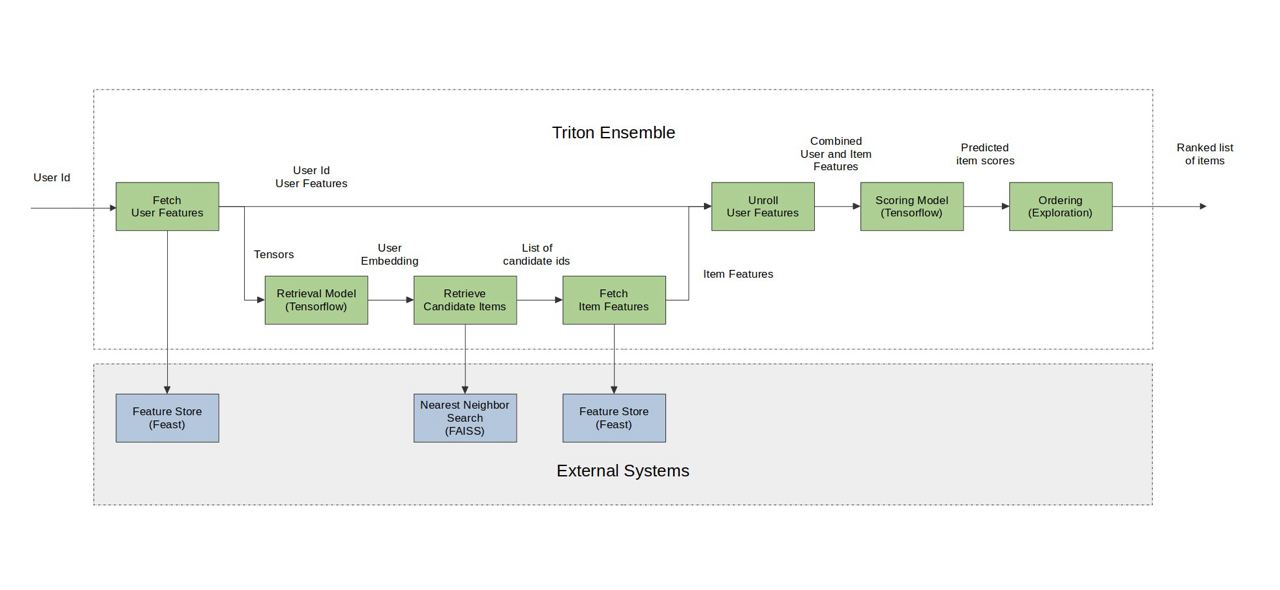
\includegraphics[width=\textwidth]{assets/deployment.jpg}
    \caption{Inference Ensemble Diagram}
    \label{fig: DeploymentDiagram}
\end{figure}

Initially, the ensemble receives a user ID as input. Once received, Triton starts executing the ensemble pipeline step by step, which consists of the following steps:

\subsection{Fetch User Features}

In this step, the server fetches the user features from the feature store (Feast). Then those features are processed by the workflow that was defined previously and saved in the model repository.

\subsection{Generate User Embedding}

Once the server has the user features, it uses them to generate a user embedding. 
It loads the query tower of the retrieval model, which is responsible for generating the user embedding. 

\subsection{Retrieve Candidate Item IDs}

During inference (online), using two separate towers to retrieve the candidate items for each customer is not efficient.~\cite{NvidiaFeatureStores}

\subsubsection{ANN (Online Retrieval)}

To reduce the latency of the responses, the system uses only the customer tower to generate the embeddings of the customers,
after that, an ANN search algorithm is used to retrieve the candidate products from the item embedding store by doing an ANN search using the customer embedding, 
in other words, calculates the similarity between the customer embedding and item embeddings then retrieves the top hundred or so nearest items.


The server uses FAISS~\cite{Faiss} to perform the nearest neighbor search computation on a GPU.
Faiss returns a list of candidate item IDs based on their embedding similarity to the user embedding.

\subsubsection{Fetch Item Features}

Once the candidate item IDs are retrieved, the server fetches the item features from the feature store (Feast) based on the candidate item IDs.
Then, loads the preprocessing workflow from the model repository and feeds those features into the workflow to process and tag them.

\subsection{Unroll User Features}

After fetching the item features, the server combines them with the user features using an operation called "Unrolling", where the user features are repeated for each item in the candidate list as shown in Figure \ref{fig: UnrollUserFeatures}.

\begin{figure}[H]
    \centering
    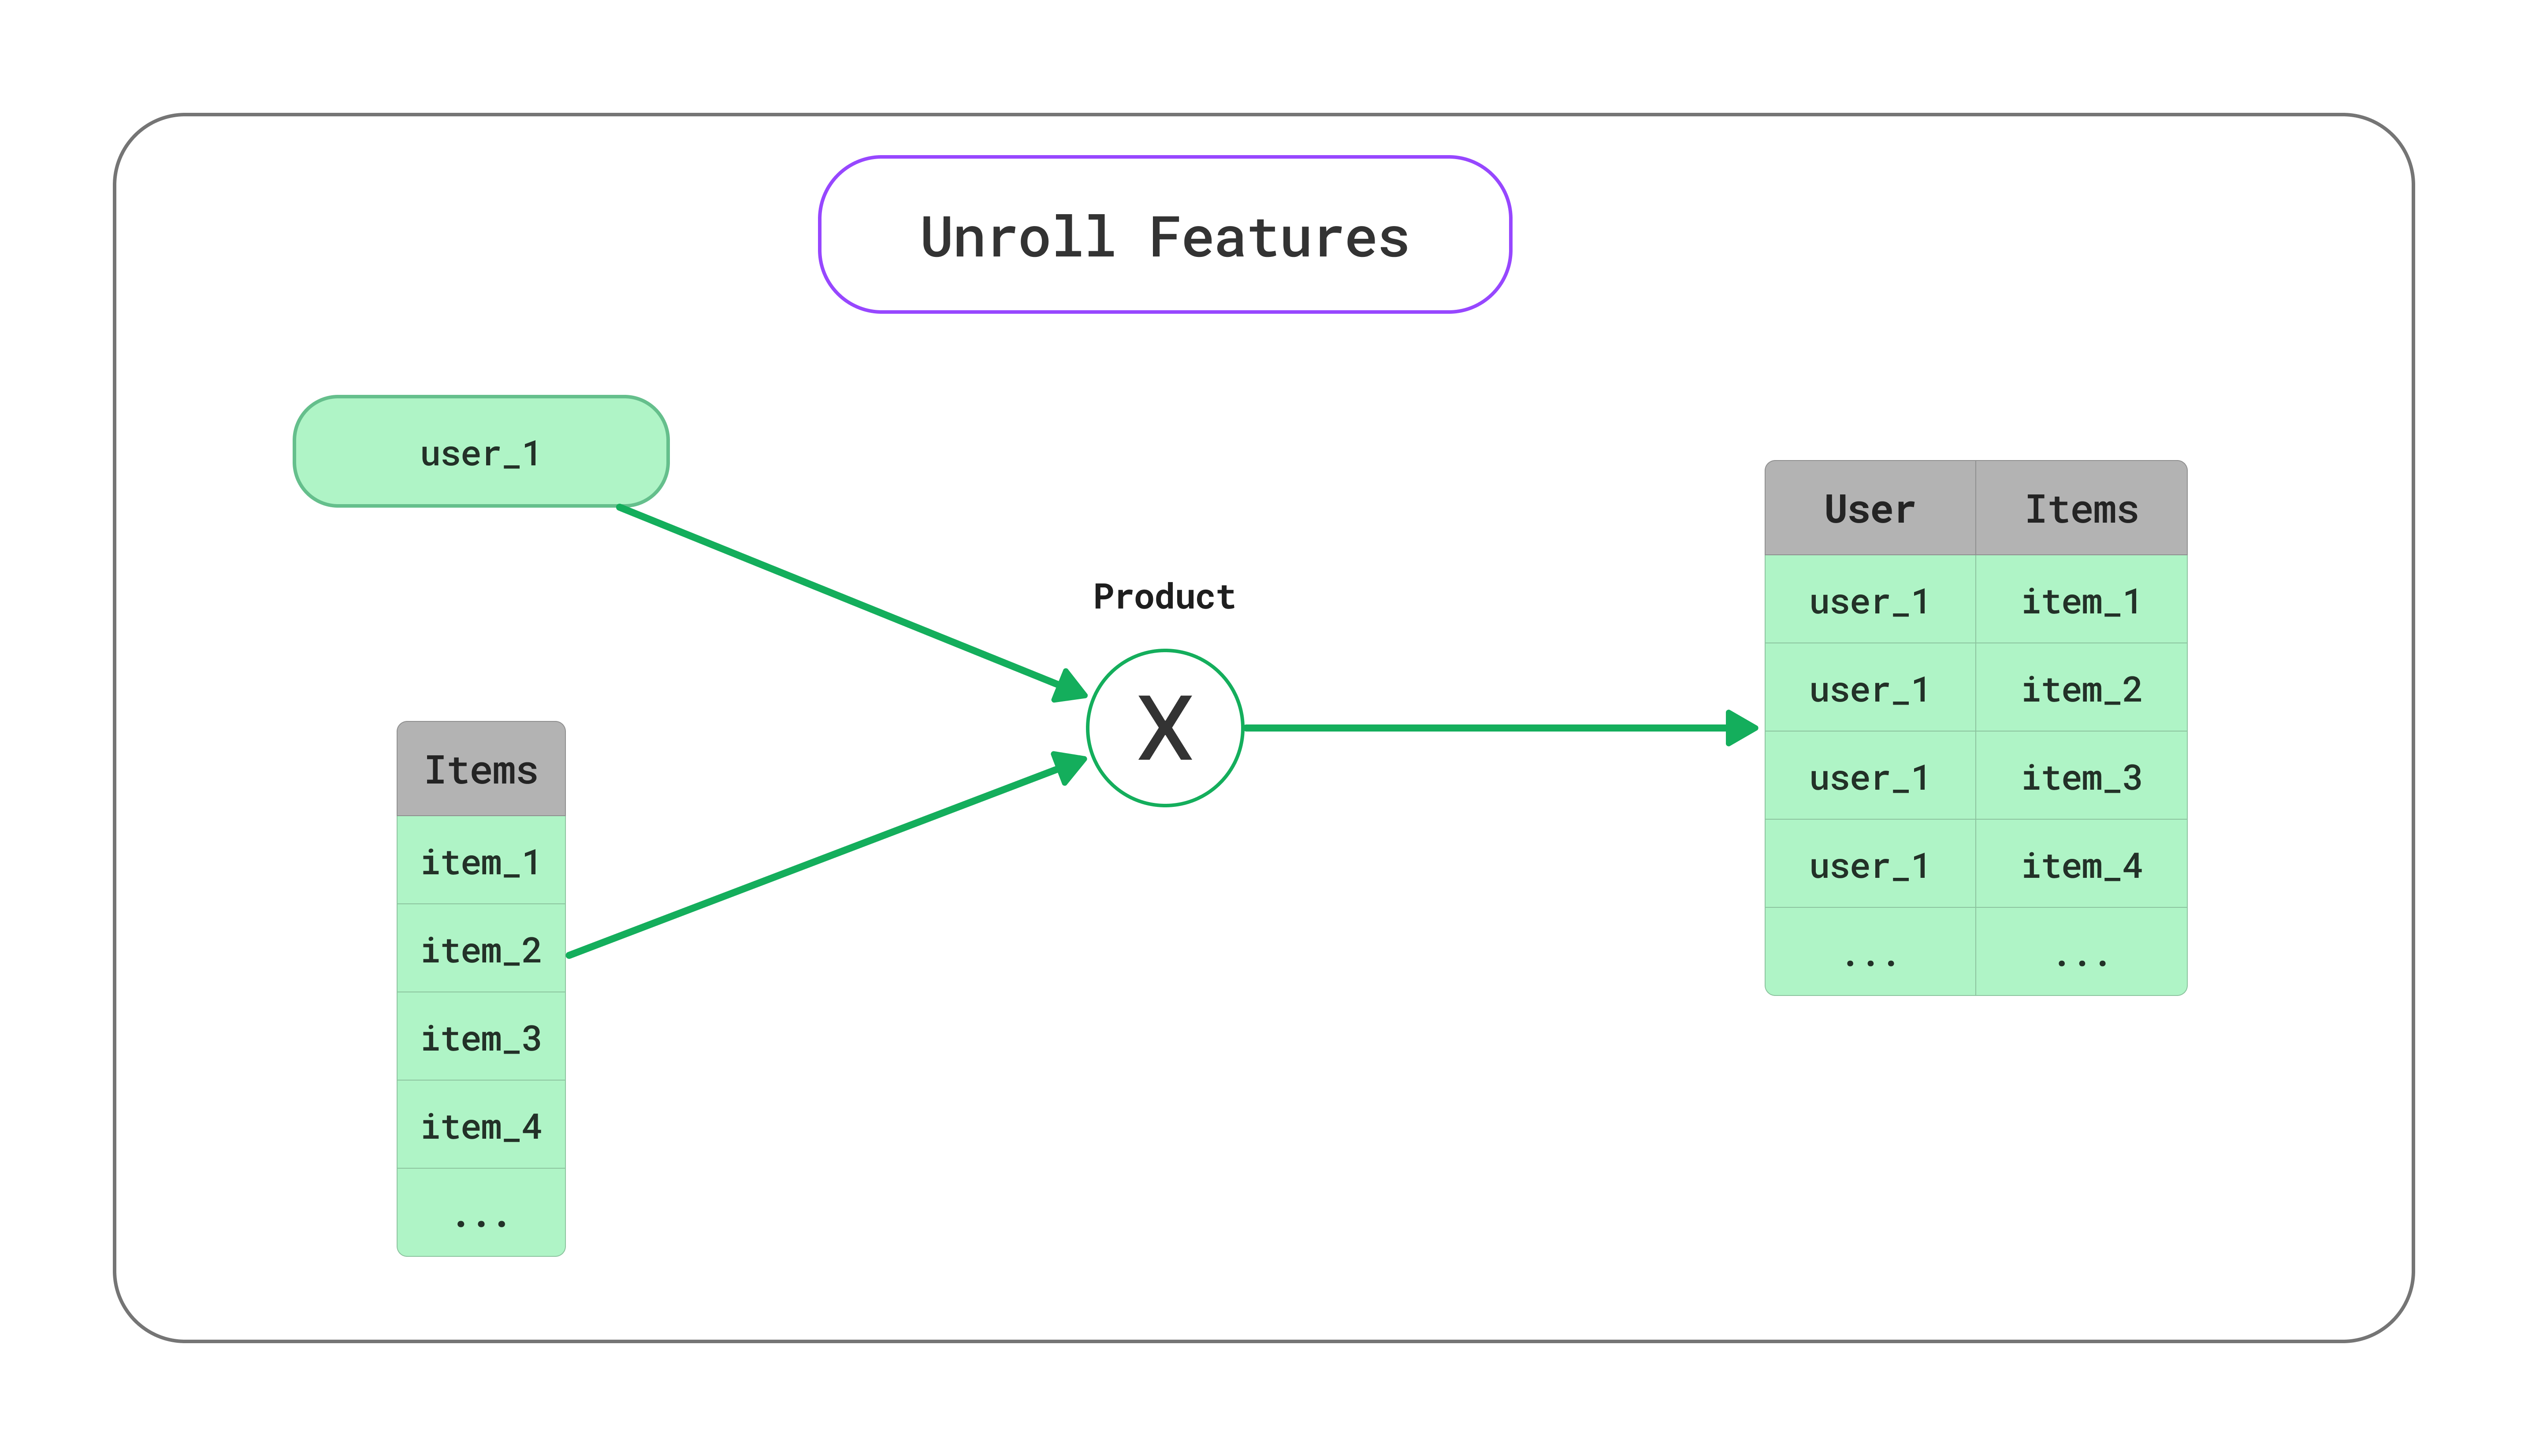
\includegraphics[width=\textwidth]{assets/Unroll Features.png}
    \caption{Unroll User/Item Features}
    \label{fig: UnrollUserFeatures}
\end{figure}


\subsection{Rule Based Filtering (Filtering)}

After retrieving the candidate products for each customer, the system filters the candidate products according to business rules and constraints.
In an e-commerce platform, the business rules and constraints usually include the availability of the products, the customer's location and shipping availability to it.


The filtering workflow is implemented using NVTabular~\cite{MerlinNVTabular}, and the workflow is stored in the model repository.

In production, the filtering workflow is deployed with the deep learning ranking model in the same container.


\subsection{Score Items}

The server loads the DLRM model from the model repository and then feeds the combined user and item features into the model to get the relevance scores.

The DLRM is deployed using Nvidia Triton Inference Server~\cite{Triton} on a Merlin Inference container~\cite{NvidiaMerlinInference} from Nvidia's NGC~\cite{NvidiaNGC}, Which is deployed on AWS SageMaker.
AWS SageMaker~\cite{AwsSageMaker} automatically scales the number of instances of the Triton Inference Server based on the load.

This step outputs a list of item IDs and their corresponding relevance scores (click probability).

\subsection{Order Items and Softmax Sampling}

Finally, the server uses the relevance scores to rank the items in the candidate list. 

\subsubsection{Softmax Sampling}

Instead of returning the top N items, the server uses a softmax sampling technique to sample items from different positions in the ranked list.
The sampling is important to ensure diversity in the recommendations and to avoid recommending the same items to all users or the same items to the same user in different sessions.
In addition, sampling helps the user explore new categories of items and interact with them which tells the system more about the user preferences.

This step is the last step in the ensemble pipeline, and the server returns the sampled items to the client.

\subsubsection{Business Rules Ordering}

In most e-commerce platforms, the business rules require the system to promote some products,
promoting products means putting them on top of the list if they exceed a certain threshold score.

The following equation represents the final score of the product which is used to order the products:

\textbf{New score = { 1.0  if (IsPromoted AND RankingScore >= Threshold) else RankingScore }}

This step is implemented in the API gateway since the number of products to be ordered after the ranking is very small and doesn't need an accelerated infrastructure.


\section{Similar Products Inference Ensemble}

This section describes the ensemble that generates similar products to a given product.
The ensemble should receive a product ID as input and return a list of similar products to the client.

The ensemble pipeline is similar to the customer recommendation ensemble pipeline, but instead of using the user features, the server uses the item features to generate the embedding query and it retrieves the candidate items based on the similarity between the wanted item embedding and other item embeddings in the item embedding store.

After the candidate items IDs are retrieved, the ensemble follows the same steps as the customer recommendation ensemble to rank, filter, score, and order the items.